\documentclass[parskip=full]{scrartcl}

\pdfoutput=1

\title{Small Data Oversampling  \\ \LARGE{Improving small data prediction accuracy using the Geometric SMOTE algorithm}}

\author{
	Georgios Douzas\(^{1}\), Fernando Bacao\(^{1*}\), Maria Lechleitner\(^{1}\) 
	\\
	\small{\(^{1}\)NOVA Information Management School, Universidade Nova de Lisboa}
	\\
	\small{*Corresponding Author}
	\\
	\\
	\small{Postal Address: NOVA Information Management School, Campus de Campolide, 1070-312 Lisboa, Portugal}
	\\
	\small{Telephone: +351 21 382 8610}
}

\usepackage{breakcites}
\usepackage{float}
\usepackage{graphicx}
\usepackage{geometry}
\geometry{
	a4paper,
	total={170mm,257mm},
	left=18mm,
	right=18mm,
	top=8mm,
}
\usepackage{amsmath}
\newcommand{\inlineeqnum}{\refstepcounter{equation}~~\mbox{(\theequation)}}
\usepackage{enumitem}
\usepackage[ruled,vlined]{algorithm2e}
\usepackage{booktabs}
\usepackage{pgfplotstable}
\pgfplotsset{compat=1.14}
\usepackage{longtable}
\usepackage{tabu}
\usepackage{hyperref}
\date{}

\begin{document}

\maketitle

\begin{abstract}
Abstract
\end{abstract}

\section{Introduction}
One of the key problems in supervised learning is the insufficient size of data
sets \cite{Niyogi.1998}. The limited availability of training sample sets can be
caused by different factors. Data is becoming an increasingly expensive resource
\cite{Li.2007} as the process to retain data is getting more complex due to
strict privacy regulations such as the General Data Protection Regulation (GDPR)
\cite{EuropeanCommission.2019}. Additionally, the small dataset problem can be
found in numerous industries where organizations simply do not have access to a
reasonable amount of data: manufacturing industries are usually dealing with
small data in early stages of product developments; health care organizations
have to work with different kinds of rare diseases, where very few records
around the world are available; and in financial industries, fraud detection is
an important issue with only few examples for cases of violence
\cite{AbdulLateh.2017}.

A sufficient training sample set is one of the basic assumptions in Machine
Learning \cite{Ivanescu.2006}. However, in the context of computational learning
theory, small sample size is one of the encountered difficulties among
measurement error, model fitting and characteristics of predictors
\cite{AbdulLateh.2017}. Small datasets do not provide an unbiased representation
of the reality due to a loose data structure with many information gaps. This
lack of learning information causes a major issue in the performance of the
machine learning algorithm \cite{Lin.2018}. Consequently, the knowledge gained
from prediction models with small sample sizes is considered unreliable as well
as imprecise and does not lead to a robust classification performance
\cite{AbdulLateh.2017}.

The size of data is considered in two ways: first, the insufficiency of data
belonging to one class (imbalance data problem); and second, the insufficiency
in the whole data (small dataset problem) \cite{Sezer.2014}. In both cases, a
small training sample set does not provide enough information to a machine
learning model to obtain a stable learning accuracy \cite{Tsai.2008}. A
theoretical explanation of “small” can be found in statistical learning theory
by Vapnik. A sample size is defined as small, if the ratio between the number of
training samples and Vapnik-Chervonenkis (VC) dimensions is less than 20. Where
the VC dimension is the maximum number of vectors that can be separated into two
classes in all possible ways by a set of functions \cite{Vapnik.2008}. 

\begin{figure}[h]
	\centering
	\includegraphics[width=0.6\linewidth]{"./resources/vc_dimension"}
	\caption{Example of VC Dimension \cite{Vapnik.2008}}
	\label{fig:vc-dimension}
\end{figure}

In the figure presented above, the VC dimension is equal to 3, since the lines
in the graph can shatter three vectors (see graphic to the left). As it is
demonstrated in the graph on the right side, the vectors z{\tiny 2} and z{\tiny
4} cannot be separated by a line from the vectors z{\tiny 1} and z{\tiny 3}
\cite{Vapnik.2008}.

Under-representation in the sample set can be solved in different ways, whereas
the use of synthetic data derived from existing (real) observations is a
promising approach \cite{Sezer.2014}. Thus, techniques to artificially add
hidden information to extend the sample size and eventually improve
classification results of the algorithm are strongly requested. However, it is
important to consider that virtual data samples are not necessarily representing
the population, as they are artificially created. Taking this into
consideration, the challenge in virtual data generation is to create data which
extends the actual data without creating noise \cite{Li.2006}. 

\begin{figure}[h]
	\centering
	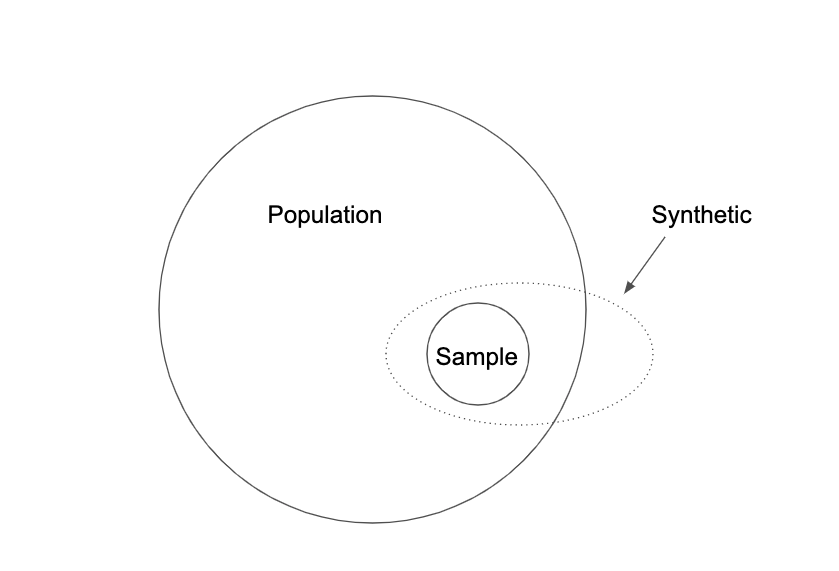
\includegraphics[width=0.35\linewidth]{./Resources/relationship}
	\caption{Relationship between population, actual data and virtual data \cite{Li.2006}}
	\label{fig:relationship}
\end{figure}

The next sections will describe an effective way to tackle this problem. First,
the previously studied solutions are reviewed. The related work in Chapter 2 is
followed by the detailed description of the proposed method, the research
methodology and the experimental results. Finally, the paper is concluded by an
analysis of the experiments in Section 6.

\section{Related Work}
Several data pre-processing methods to handle small dataset problems have been
presented in the research community. In this section, the most important
approaches are reviewed and the state-of-the-art to improve small dataset
learning is pointed out. In the first section fuzzy theory is presented, which
is the most mentioned group of techniques to solve a small dataset problem.
Furthermore, Resampling Mechanisms are pointed out which mainly address
bootstrapping techniques. Finally, oversampling techniques are reviewed which
can be a potential solution for increasing the sample size of small datasets.

\subsection{Fuzzy Theories}
In order to build an accurate prediction model, a large sample of the population
is required to train the model. When the dataset is small, artificial data
generation approaches can be employed to increase the sample size.  Many
techniques presented in the literature are based on fuzzy theories
\cite{AbdulLateh.2017}. The fuzzy set theory provides a strict mathematical
framework to generalize the classical notion of a dataset. It gives a wider
scope of applicability, especially in the fields of information processing and
pattern classification \cite{Zimmermann.2010}. Based on this concept, several
methods have emerged in the last decade to estimate or approximate functions
which are generating more samples for sparse training sets.

One of the most effective methods to improve the learning performance of
prediction models is artificial sample generation. It is proven that the
accuracy of the learning algorithm is improved, when increasing the sample size
of training sets \cite{AbdulLateh.2017}. Thus, the gaps between observations
(information gaps) will be filled with artificial samples derived from the
population to feed the algorithm with a more complete representation of the
reality.

\begin{figure}[h]
	\centering
	\includegraphics[width=0.6\linewidth]{"./Resources/small_data_distribution"}
	\caption{Distribution of a small dataset}
	\label{fig:small-data-distribution}
\end{figure}

The concept of artificially creating data, called Virtual Sample Generation
(VSG), was originally proposed by \cite{Niyogi.1998}. The idea is to create
additional examples from the current set of real-life examples by using prior
information gained from the available data. The introduction of virtual examples
expands the effective training set size and can therefore solve the learning
problem. \cite{Niyogi.1998} proved that the process of creating artificial
samples is mathematically equivalent to incorporating prior knowledge. They
demonstrate the concept on object recognition by mathematically transforming the
views of 3D-objects. These new views are called ‘virtual samples’ which
application extends information and results in successful generalization. 

Based on this theory, several closely related studies were developed for
manufacturing environments. The first method to overcome scheduling problems due
to the lack of data in early stages of manufacturing systems was the creation of
a Functional Virtual Population (FVP) by \cite{Li.2003}.  Their study expands
the original sample size instead of simply adding new data. The idea is to
create a number of virtual samples within of a newly defined domain range. The
method involves a highly manual process, however, the application of FVP
dramatically improved the classification accuracy of a Neural Network. In 2004,
the idea of fuzzifying information to extend a small dataset was used to develop
the Diffusion-Neural-Network (DNN) method \cite{Huang.2004}. It combines the
principle of information diffusion by \cite{Huang.1997} with traditional Neural
Networks to estimate functions. The information diffusion method partially fills
the information gaps by using fuzzy theories to represent the similarities
between samples and subsequently derive new samples. 

The researchers \cite{Li.2006b} further examined possible methods to learn
scheduling knowledge with rare data in early stages of manufacturing systems.
They developed a new data fuzzification technique called mega-fuzzification and
combined it with a data trend estimation procedure to systematically expand the
small dataset. The method fuzzifies the dataset as a whole and expands it in
regard of a previously defined data trend. The results of this study show high
learning accuracy and denote the method as a reliable and applicable approach in
the business marketplace. However, it is considered as an unfavorable
technique, because there is a lack of theoretical basis in the determination of
domain ranges. 

In order to fully fill the information gaps, a technique which diffuses the
sample set one for one was introduced by \cite{Li.2007}. To avoid the
over-estimation, their concept is to combine data trend estimation with a mega
diffusion technique to estimate the domain range. The method is called
Mega-Trend-Diffusion (MTD) and diffuses a set of data instead of each sample
individually. For example, two samples m and n (Figure 4) are diffused
simultaneously into one function with their borders a and b. To estimate a and
b, the algorithm takes the minimum and maximum values of the dataset and counts
the number of data points which are smaller or greater than the average of the
values. This takes the skewness in the distribution of the data and the domain
range into consideration when calculating new samples. The triangular shape of
figure 3 represents the membership function which shows the similarities between
samples. M and n are the samples and their heights are the possible values of
the membership function.

\begin{figure}[h]
	\centering
	\includegraphics[width=0.7\linewidth]{"./Resources/mtd_function"}
	\caption{MTD function}
	\label{fig:mtd-function}
\end{figure}

After estimating the domain range between a and b, samples are randomly produced
within this area by using a common diffusion function. The artificial samples
are then trained with a Back-propagation Neural Network (BPNN) like
\cite{Huang.2004} originally proposed. This technique is seen as an improvement
of DNN and was initially developed to improve early flexible manufacturing
system scheduling accuracy. In further research, MTD is widely used as a
synthetic sample generation method and is recognized as an effective way to deal
with small dataset problems \cite{AbdulLateh.2017}. However, MTD only considers
the data for independent attributes and does not deal with their relationships. 

Therefore, a genetic algorithm based virtual sample generation (GABVSG) was
developed. The novel method takes the relationship among the attributes into
account and explores the integrated effects of attributes instead of dealing
with them individually. This algorithm is performed in three steps: Samples are
randomly selected to determine the range of each attribute by using MTD
functions. Next, a Genetic Algorithm is applied to find the most feasible
virtual samples. Finally, the average error of these new samples is calculated.
The results outperformed the ones using MTD and also showed better performance
in prediction than in case of no generation of synthetic samples \cite{Li.2014}.

The above presented fuzzy-based algorithms can only deal with numeric
attributes. When the dataset contains nominal features, resampling mechanisms
have to be considered such as Bootstrap. Although it is possible to transform
nominal values into binary ones, the relationship between the values of the
attributes would get lost \cite{Tsai.2008}. 

\subsection{Resampling Mechanism}

An alternative approach to fuzzy theories is the statistical method called
Bootstrap to increase the amount of observations. Bootstrap is the most
well-known synthetic sample generation method which uses a statistical
resampling mechanism to create new observations \cite{AbdulLateh.2017}. It forms
new training sets by replacing the original datasets, which is the main
difference to the previously presented techniques. Thus, the amount of
information is not increased since the Bootstrap procedure only enlarges the
number of obtained observations. According to \cite{Tsai.2015}, it is seen as a
not very favorable technique, because it aims to increase the amount of
obtained observations rather than filling the information gaps. However, it was
successfully applied when solving the limited data problem in batch process
industries \cite{Ivanescu.2006} and in improving the prediction accuracy of
bladder cancer cells \cite{Chao.2011} for example. \cite{Ivanescu.2006} use the
principle of Bootstrap for generating additional job sets. In general, Bootstrap
implies randomly re-sampling the original observations with replacement.
However, rather than re-sampling the job sets, this technique uses the
individual jobs to construct new job sets. After generating artificial job sets,
the original job sets are joined which forms the new training set. Their study
shows that this approach works better than the traditional Artificial Neural
Network (ANN).

On the other hand, \cite{Chao.2011} use Bootstrap to increase the sample size on
a subset of the original dataset. The algorithm splits the dataset into only
five to 30 data points for training. Then the Bootstrap procedure is applied to
acquire a virtual sample for each datapoint of the subset. Subsequently, this
step it is repeated until it reaches 100 new artificial samples. The original
subset is joined with the new bootstrapped 100 samples and used to train the
ANN. The entire remaining data of the original subset (5 to 30 observations) is
used for validation afterwards. This technique outperforms the ANN.

\subsection{Oversampling Techniques}

A different approach to fill information gaps is synthetic oversampling of the
training set. Oversampling is an artificial data generation strategy originally
developed for imbalanced datasets. The research community is different to the
one mentioned in the previously presented methods. Their work is not related
yet, but it appears to have a high potential in future research. In Imbalanced
Learning, the classes of the given dataset are significantly skewed in a sense
that there is a difference between examples of different classes. This means,
that the dataset has a large number of observations in one class and a very
small number of observations in the other class or classes. This is an
unfavorable situation for the algorithm to learn and should be solved in the
data pre-processing phase. In practice, the imbalanced dataset problem is are
very common issue in Supervised Learning. Especially, in the fields of fraud
detection, product categorization and disease diagnosis an imbalanced dataset is
the norm rather than the exception \cite{He.2013}. 

\subsubsection{SMOTE}

There are several methods presented in the literature to tackle this problem.
One of the first and most popular methods is the synthetic minority
over-sampling technique (SMOTE). SMOTE works on the idea of k-nearest
neighbors. It generates synthetic data around vectors between the minority
class instances and their nearest neighbors \cite{Chawla.2002}. A visual
representation of the concept can be found in figure 5.

\begin{figure}[h]
	\centering
	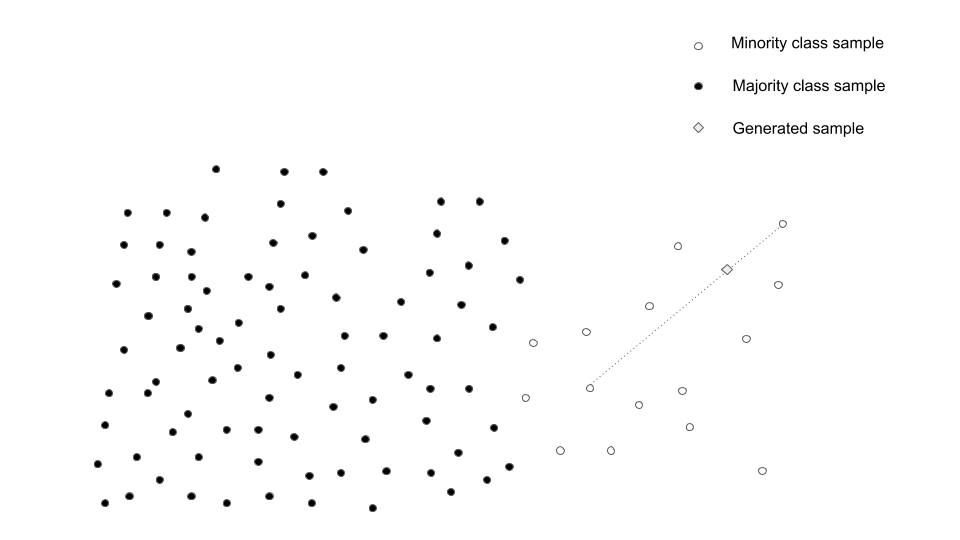
\includegraphics[width=0.5\linewidth]{./Resources/smote}
	\caption{Concept of SMOTE}
	\label{fig:smote}
\end{figure}

The algorithm is considered as a standard framework for pre-processing
imbalanced datasets due to its simplicity and as well as its robustness.
Numerous variations of SMOTE have been developed which declares SMOTE as the
foundation of synthetic sample generation when it comes to imbalanced
classification problems \cite{Fernandez.2018}. However, the algorithm faces some
limitations when it comes to the sample generation process. In practice, the
separation between majority and minority class clusters is often not clearly
definable. Thus, noisy samples may be generated when a minority sample lies in
the region of the majority classes. Figure 7 presents a scenario where a
minority instance is generated within the majority region (noisy sample).

\begin{figure}[h]
	\centering
	\includegraphics[width=0.6\linewidth]{"./resources/noisy_examples"}
	\caption{Generation of noisy examples}
	\label{fig:noisy-examples}
\end{figure}

Furthermore, redundant instances may be generated within dense minority regions.
They do not add any relevant information to the classifier and may lead to
overfitting. Figure 8 demonstrates an example where a minority class instance is
generated in a dense minority class. This new observation belongs to the same
dense cluster as the original and is therefore less useful. 

\begin{figure}[h]
	\centering
	\includegraphics[width=0.6\linewidth]{"./Resources/redundant_examples"}
	\caption{Generation of redundant examples}
	\label{fig:redundant-examples}
\end{figure}

Although SMOTE is recognized as a oversampling technique for imbalanced
datasets, it is also used for solving the small dataset problem \cite{Li.2018}.
By performing simple adjustments in the algorithm, it successfully fills the
information gaps with synthetic samples. However, it did not achieve the best
results within the study.

\subsubsection{G-SMOTE}

In consideration of the limitations of SMOTE, the novel data generation
procedure Geometric SMOTE (G-SMOTE) has been presented by \cite{Douzas.2017}.
G-SMOTE is an extension of the SMOTE data generation mechanism and can be seen
as a substitute. The main difference to SMOTE is that the novel method
significantly broadens the options for data generation. Instead of connecting
the minority sample and its nearest neighbor with a line segment (hypersphere),
the instances are generated in a geometrical region (hyper-spheroid) around the
minority sample. 

\begin{figure}[h]
	\centering
	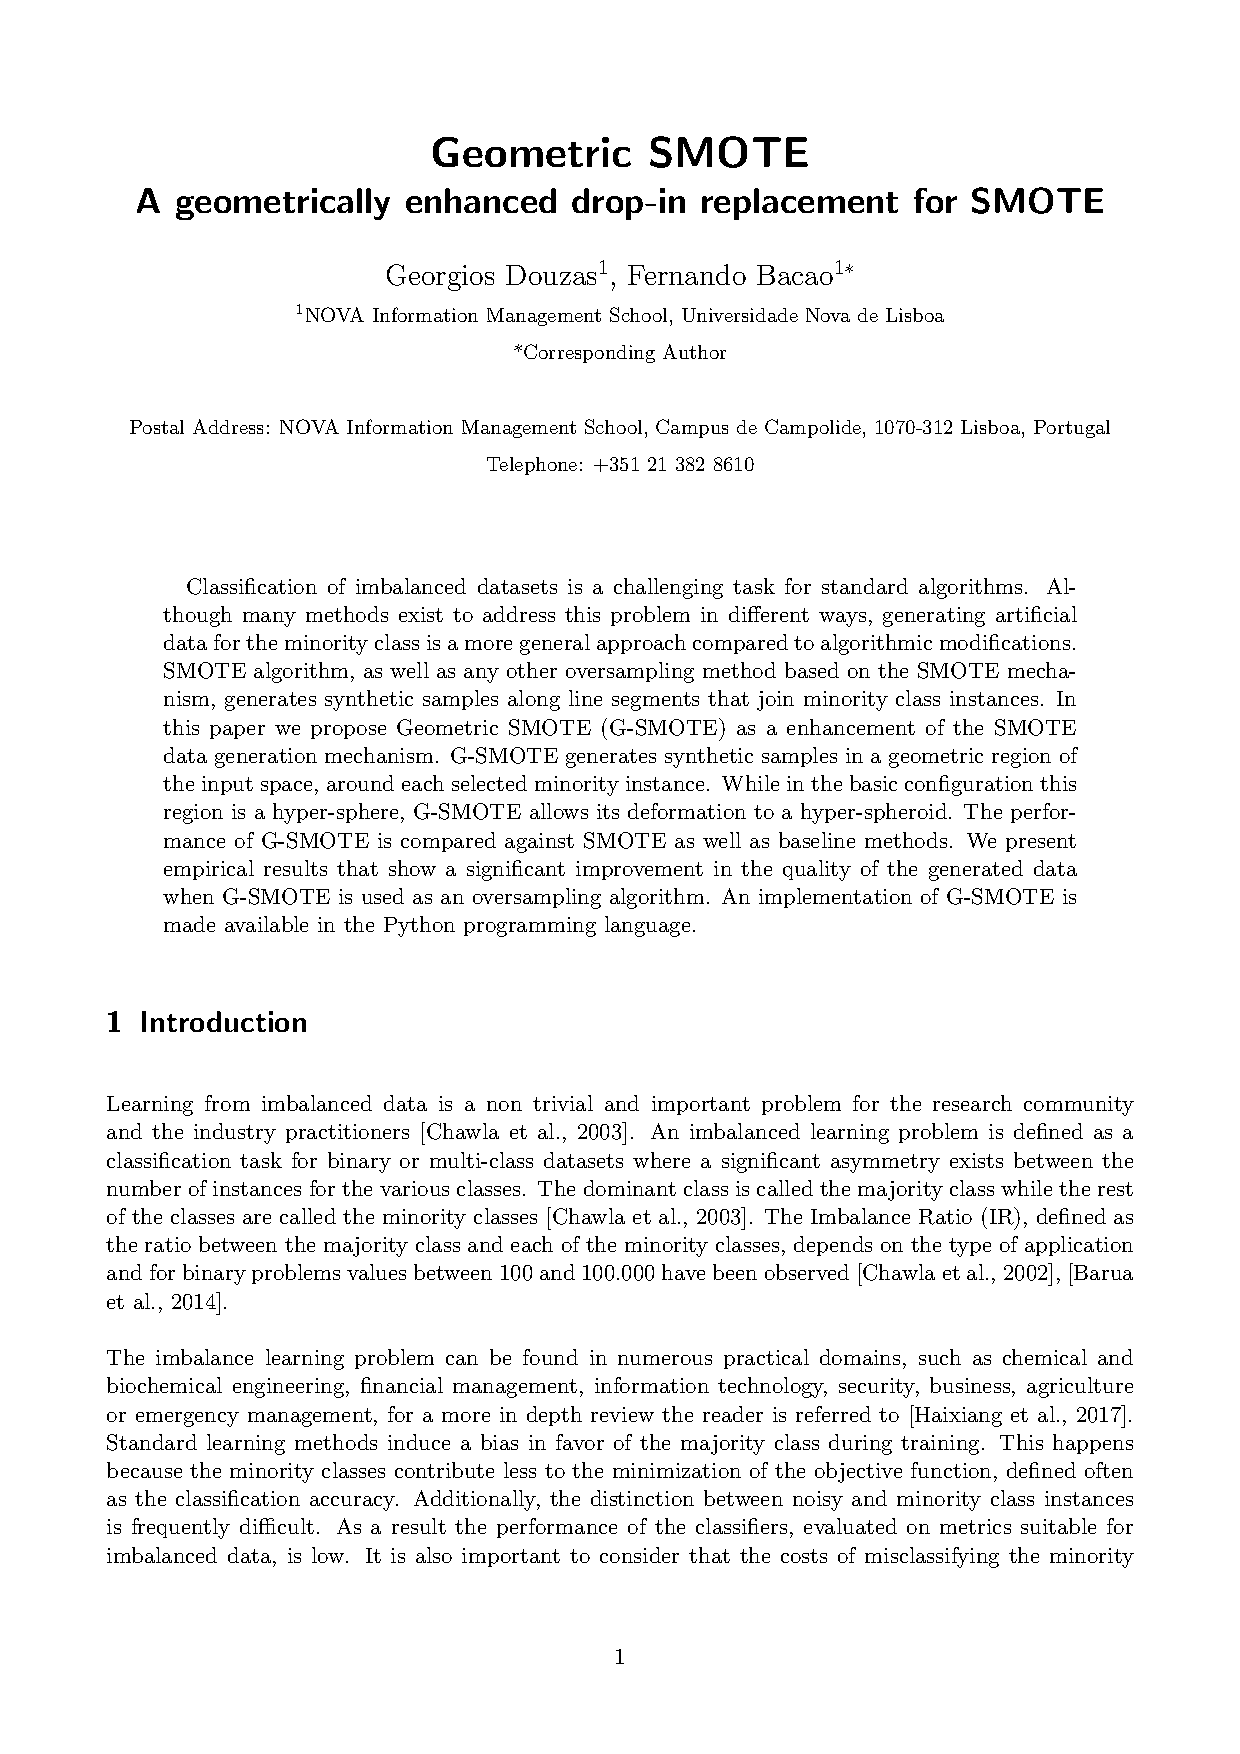
\includegraphics[width=0.5\linewidth]{./resources/gsmote}
	\caption{Concept of G-SMOTE}
	\label{fig:gsmote}
\end{figure}

Hence, it is recognized as a generalization of SMOTE, as it significantly
extends the input space for data generation. The main achievement of the novel
algorithm is that it solves the limitations of SMOTE mentioned above. G-SMOTE
defines a safe area around each minority class instance which prevents the
algorithm from creating noisy samples. Also, it increases the variety of
generated samples by expanding the minority class area with a hyper-spheroid
instead of a hypersphere. These modifications proof their refinement in
experiments with 69 imbalanced datasets and four classifiers such as Logistic
Regression (LR), K-Nearest Neighbors (KNN), Decision Tree (DT) and Gradient
Boosting (GBC). The results show that G-SMOTE is outperforming SMOTE, Random
Oversampling and the case of no oversampling at all, across all classifiers and
performance metrics.  

Various methods to deal with small datasets or a small representation of a class
have been presented in this section. It has been proven, that all cases with
artificially increased sample size seem to enhance the prediction performance of
the conventional classifier. Thus, data pre-processing of a small or imbalanced
dataset by increasing the sample size is an important task in the area of
Machine Learning \cite{Ruparel.2013}.

\section{Proposed Method}

Adapted GSMOTE for Small Dataset Learning (describe algorithm)

\section{Research Methodology}

\subsubsection{Experimental Data}
\subsubsection{Evaluation Measures}
\subsubsection{Machine Learning Algorithms}
\subsubsection{Experimental Procedure}
\subsubsection{Software Implementation}

\section{Results and Discussion}
\subsection{Comparative Presentation}
\subsection{Statistical analysis}

\section{Conclusions}

\bibliography{references}
\bibliographystyle{apalike}

\end{document}
